\section{overview}

\begin{frame}
    \frametitle{时间序列预测定义}
    尽管有诸多因素干扰,依然有可能基于对现实现象的历史观测推导出一个模型,用来计算一定提前期的未来值。
    时间序列预测正是通过对时间序列观测值之间相互依赖性的分析,发展出动态模型,进而对时间序列的未来状态进行预测。

    \vspace*{1em}
    \textbf{时间序列预测的过程本质上是一个以历史时间序列为自变量,以未来时间序列为因变量的函数逼近过程。}

    即,给定一个历史T步的时间序列$\bm{x} = (x_1, \ldots, x_T)$,\(\x \in \mathr^{T}\),以及未来提前H步的时间序列$\bm{y} = (x_{T+1},\ldots,x_{T+H})$, \(\y \in \mathr^{H}\),时间序列预测问题可被公式化定义为:
\begin{equation*}
    \mathcal{F} : f(\bm x) + \bm e = \bm y, \label{eq:sec.intro.def}
\end{equation*}

$\mathcal{F}$是指时间序列预测模型所逼近的函数。\(f\)是指时间序列预测模型所学习出的预测函数。

\end{frame}

\begin{frame}
    \frametitle{传统时间序列预测建模技术}

    以统计学为基础的回归预测模型,通过构造历史观测值与相关因素的经验方程,对时间序列进行拟合和预测。

    \begin{itemize}
        \item 自回归(Auto-regressive,AR)模型
        \item 移动平均(Moving average,MA)模型
        \item 自回归移动平均混合(Auto-regressive moving average,ARMA)模型
        \item 整合移动平均自回归(Auto-regressive integrated moving average,ARIMA)模型
        \item 指数平滑(Exponential smoothing,ES)模型
    \end{itemize}


    归纳:
    \begin{itemize}
        \item 将时间序列数据的输入输出映射视为预定义的函数
        \item 仅适用于某一特定类型的平稳过程或非平稳过程
        \item 不能有效处理复杂非线性非平稳的时间序列预测问题
    \end{itemize}

\end{frame}

\begin{frame}
    \frametitle{机器学习预测建模技术}
    将预测问题考虑为一种以历史T步的时间序列$\bm{x} = (x_1, \ldots, x_T)$为输入,以未来提前H步的时间序列$\bm{y} = (x_{T+1},\ldots,x_{T+H})$为输出的回归问题,构造监督机制下的回归模型予以求解。
    \begin{equation*}
        f(\bm x) + \bm e = \bm y, \quad f \in \{\vartheta, \theta\}\label{eq:sec.intro.ml}.
    \end{equation*}

    \(\theta\)表示机器学习预测模型的权重参数集合,\(\vartheta\)表示定义机器学习预测模型
    与权重学习机制的超参数集合。

    \begin{itemize}
        \item \(\vartheta\)定义了机器学习预测模型的结构与权重参数的训练机制
        \item \(\theta\)表示机器学习模型中从输入变换到输出间的权重参数集合
        \item \(f \in \{\vartheta, \theta\}\)
    \end{itemize}

    \vspace{1em}
    \centering
    如何选择合适的\(\vartheta\)与\(\theta\)从而建立一个精准的预测模型\(f\)
\end{frame}

\begin{frame}
    \frametitle{ML代表模型}

    \begin{figure}
        \begin{minipage}[b]{0.45\textwidth}
            \centering
            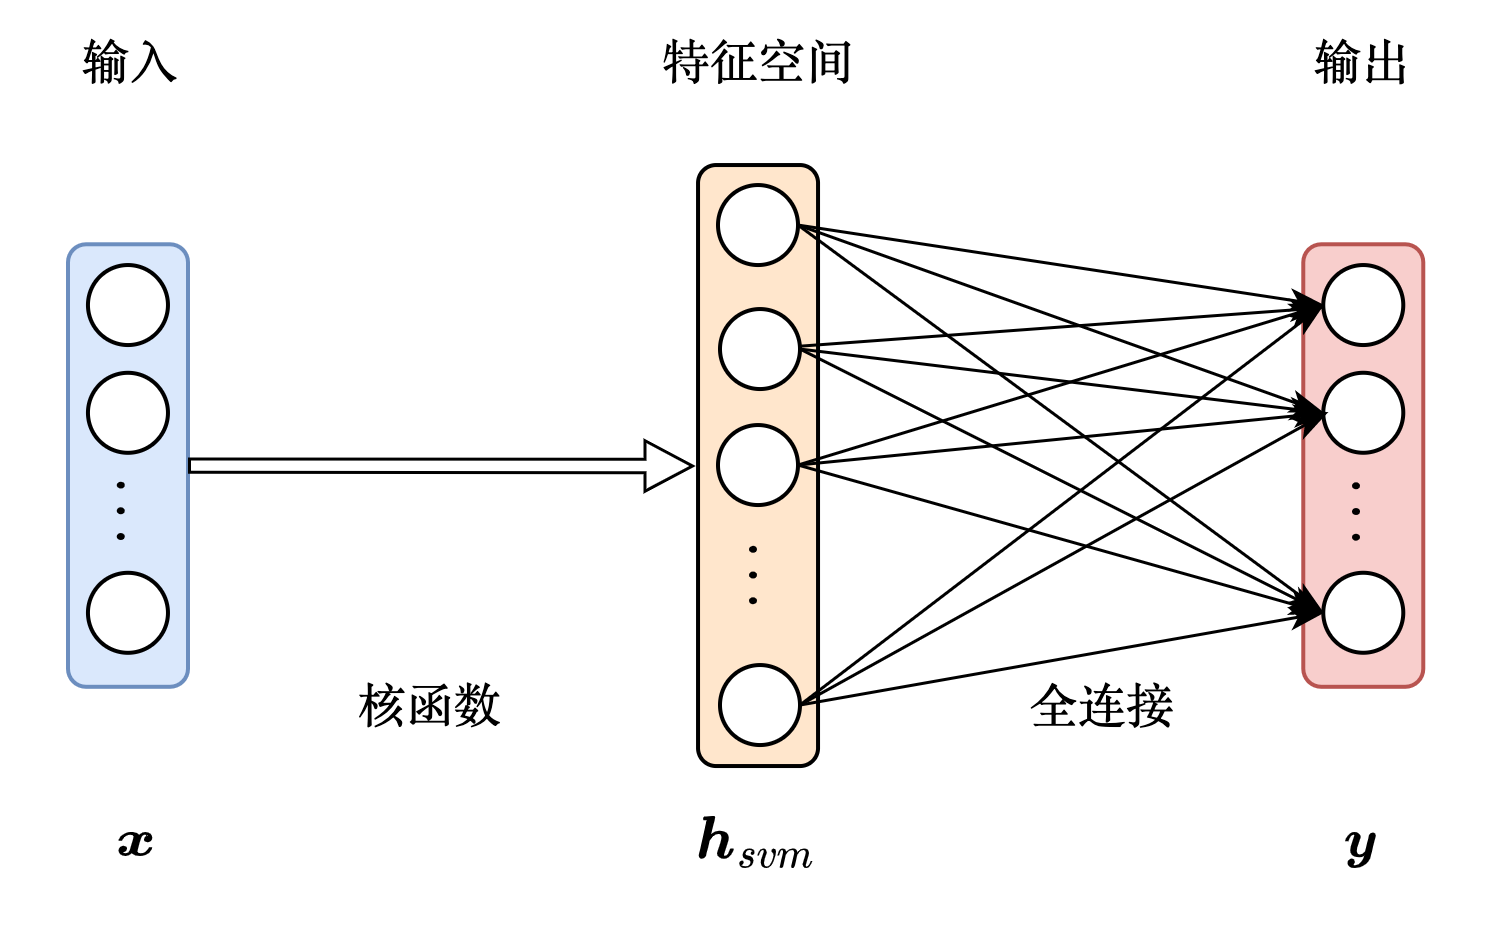
\includegraphics[width=\textwidth]{float/ch.intro/svm.png}
            \caption*{支持向量机(SVM)结构示例\label{fig:ch.intro.svm}}
        \end{minipage}
        \hfill
        \begin{minipage}[b]{0.45\textwidth}
            \centering
            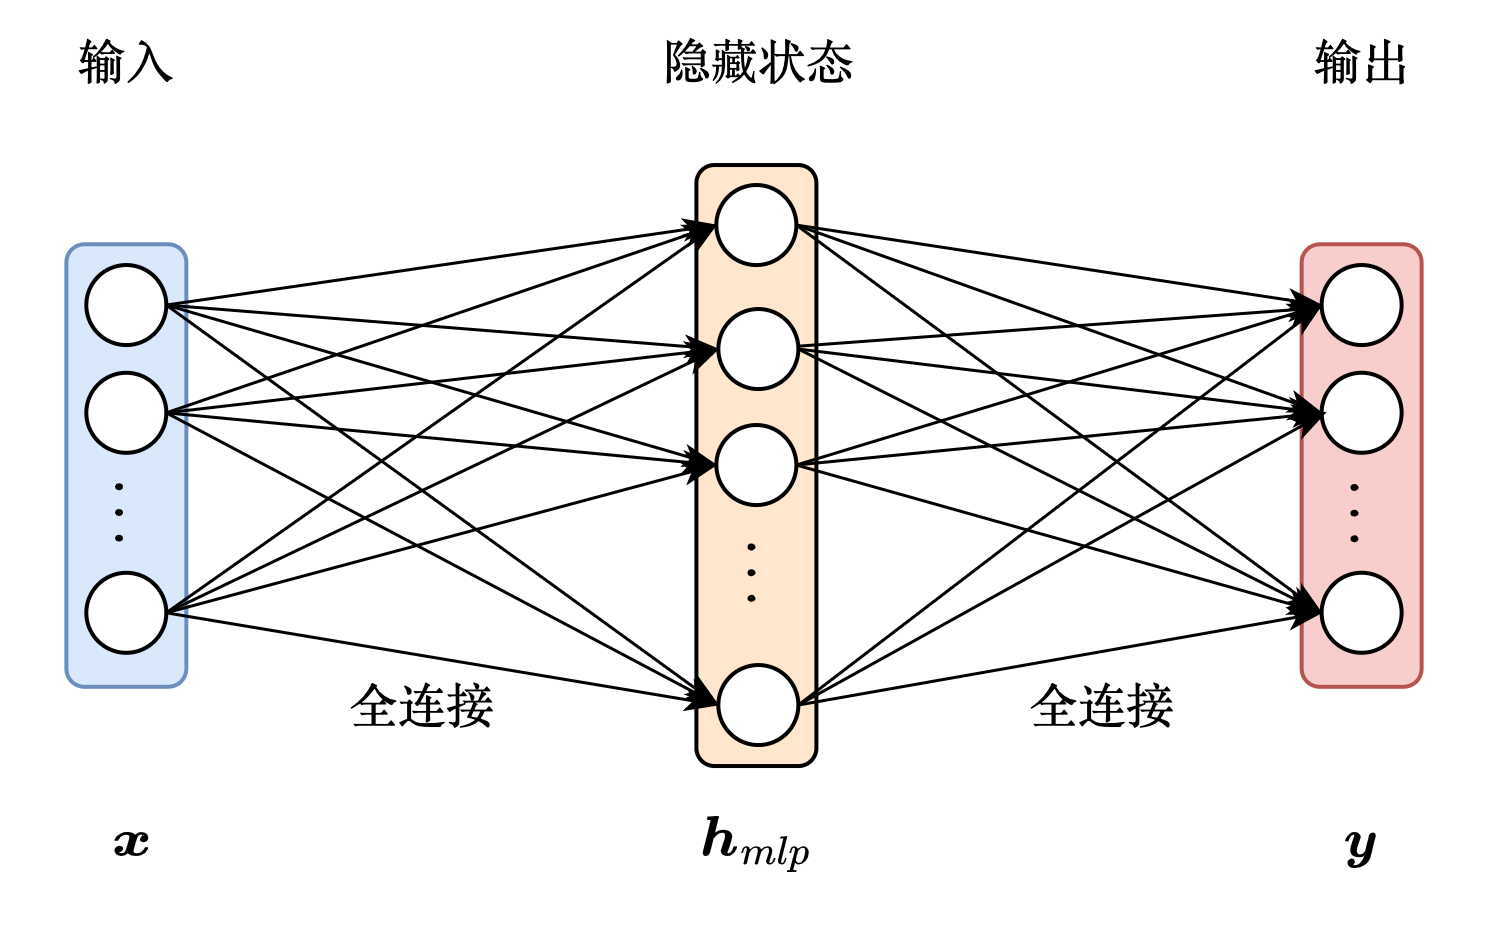
\includegraphics[width=\textwidth]{float/ch.intro/mlp.png}
            \caption*{多层感知机(MLP)结构示例\label{fig:ch.intro.mlp}}
        \end{minipage}
    \end{figure}

    以一组给定包含\(N\)个样本的时间序列数据集\(\mathbb{D} = \left\{\left(\x_{n}, \y_{n}\right) \in\left(\mathbb{R}^{T} \times \mathbb{R}^{H}\right)\right\}_{n=1}^{N}\)为例,对基于SVM与NN的预测建模技术与应用展开概述。

\end{frame}

\begin{frame}
    \frametitle{梯度下降}
    常有学者将基于梯度下降方法的神经网络模型称为反向传播神经网络(Back propagation neural network,BPNN)模型。

    \begin{itemize}
        \item 梯度下降:梯度下降训练方法中各层权重参数的优化方法
        \item 反向传播:梯度下降训练方法中计算各层权重参数梯度时所使用的链式法则梯度传导过程
    \end{itemize}

    以MLP为例:
    \begin{align*}
        \ell(\w) &= \frac{1}{N \times H} \sum^N_{n=1} \|\e_{n}\| ,\label{eq:ch.intro.mse}\\
        \e_{n} & = \y_n - f(\x_n).
    \end{align*}
    \centering
    \(\ell(\w)\)为神经网络预测模型在训练集\(\mathd\)上的MSE损失

\end{frame}

\begin{frame}
    \frametitle{梯度下降}

    核心思想:
    \begin{itemize}
        \item 基于神经网络模型中激活函数的连续性与可微性
        \item 向\(\w\)添加一个很小的动量\(\Delta_{\w}\),即\(\norm{\Delta_{\w}}\)很小,亦等价于\(\w + \Delta_{\w}\)近似\(\w\)
        \item 利用泰勒近似将复杂非凸的\(\ell(\w)\)函数优化问题当作一个简单的函数极小值问题
    \end{itemize}
    \begin{equation*}
        \ell({\w + \Delta_{\w}} ) \approx \ell({\w}) + \nabla_{\w}^{\mathrm{T}}\Delta_{\w}.
    \end{equation*}
    \(\nabla_{\w}\)表示\(\w\)在误差函数\(\w\)中的梯度。在最陡下降中,定义学习速率(Learning rate)为\(\eta \),且\(\eta  > 0\),因此:
    \begin{equation*}
        \Delta_{\w} = -\eta \nabla_{\w}. \label{eq:ch.intro.gd2}
    \end{equation*}
    当\(\eta \)足够小,可证:
    \begin{equation*}
        \ell({\w -\eta \nabla_{\w}} ) \approx \ell({\w})  -\eta  \nabla_{\w}^\trans \nabla_{\w} < \ell({\w}). \label{eq:ch.intro.lr}
    \end{equation*}
\end{frame}

\begin{frame}
    \frametitle{梯度下降的范式}

    \begin{algorithm}[H]
        \caption{神经网络模型梯度下降方法训练过程}
        % \renewcommand{\algorithmcfname}{算法}
        % \renewcommand{\algorithmicrequire}{\textbf{输入:}}
        % \renewcommand{\algorithmicensure}{\textbf{输出:}}
        \label{alg:ch.intro.gd}
        \begin{algorithmic}[1]
            \WHILE{未满足\(\vartheta\)界定的收敛条件}
            \STATE \(i\leftarrow i+1\)
            \STATE 基于\(\theta^i\),确定模型\(f \leftarrow  f \in \{\vartheta, \theta^i\}\)
            \STATE 基于数据集\(\mathd\)和模型\(f\),完成前馈过程\(f(\x)\),计算模型损失函数值\(\ell({\w}) \)
            \FOR{\(\w\) in \(\theta^i\) }
            \STATE 选取计算梯度所需的样本
            \STATE 根据反向传播链式法则计算梯度信息\(\nabla_{\w}\)
            \STATE 根据梯度下降更新公式更新权重参数\(\w\)
            \ENDFOR
            \ENDWHILE
            \RETURN {
                已完成更新过程的权重参数集合\(\theta \leftarrow \theta^i\)
            }
        \end{algorithmic}
    \end{algorithm}

\end{frame}

\begin{frame}
    \frametitle{深度学习建模方法}
    深度学习建模技术是机器学习建模技术中一类基于深度神经网络的建模方法。
    \begin{itemize}
        \item 海量数据的积累:CIFAR10,CIFAR100,ImageNet,WMT
        \item 计算能力的提升:GPU加速,分布式计算,并行计算
        \item 梯度下降的改进:SGD,Moment,Adam
        \item 通用框架的提出:TensorFlow,Pytorch
    \end{itemize}

    \begin{figure}
        \begin{minipage}[t]{0.55\textwidth}
            \begin{itemize}
                \item {
                    传统机器学习:人工经验建立特定的特征提取方法\begin{itemize}
                        \item 基于图像像素数值高斯分布描述图像特征的Fisher Vector方法
                        \item 基于语言文档内词频信息描述语句特征的词频-逆文档(TF-IDF)方法
                    \end{itemize}
                }
            \end{itemize}
        \end{minipage}
        \hfill
        \begin{minipage}[t]{0.44\textwidth}
            \begin{itemize}
                \item {
                    深度学习:依靠神经网络结构学习数据的抽象特征表示\begin{itemize}
                        \item CNN中的卷积结构
                        \item RNN中的循环结构
                    \end{itemize}
                }
            \end{itemize}
        \end{minipage}
    \end{figure}
\end{frame}

\begin{frame}
    \frametitle{深度学习示例}

    \begin{figure}[t!]
        \centering
        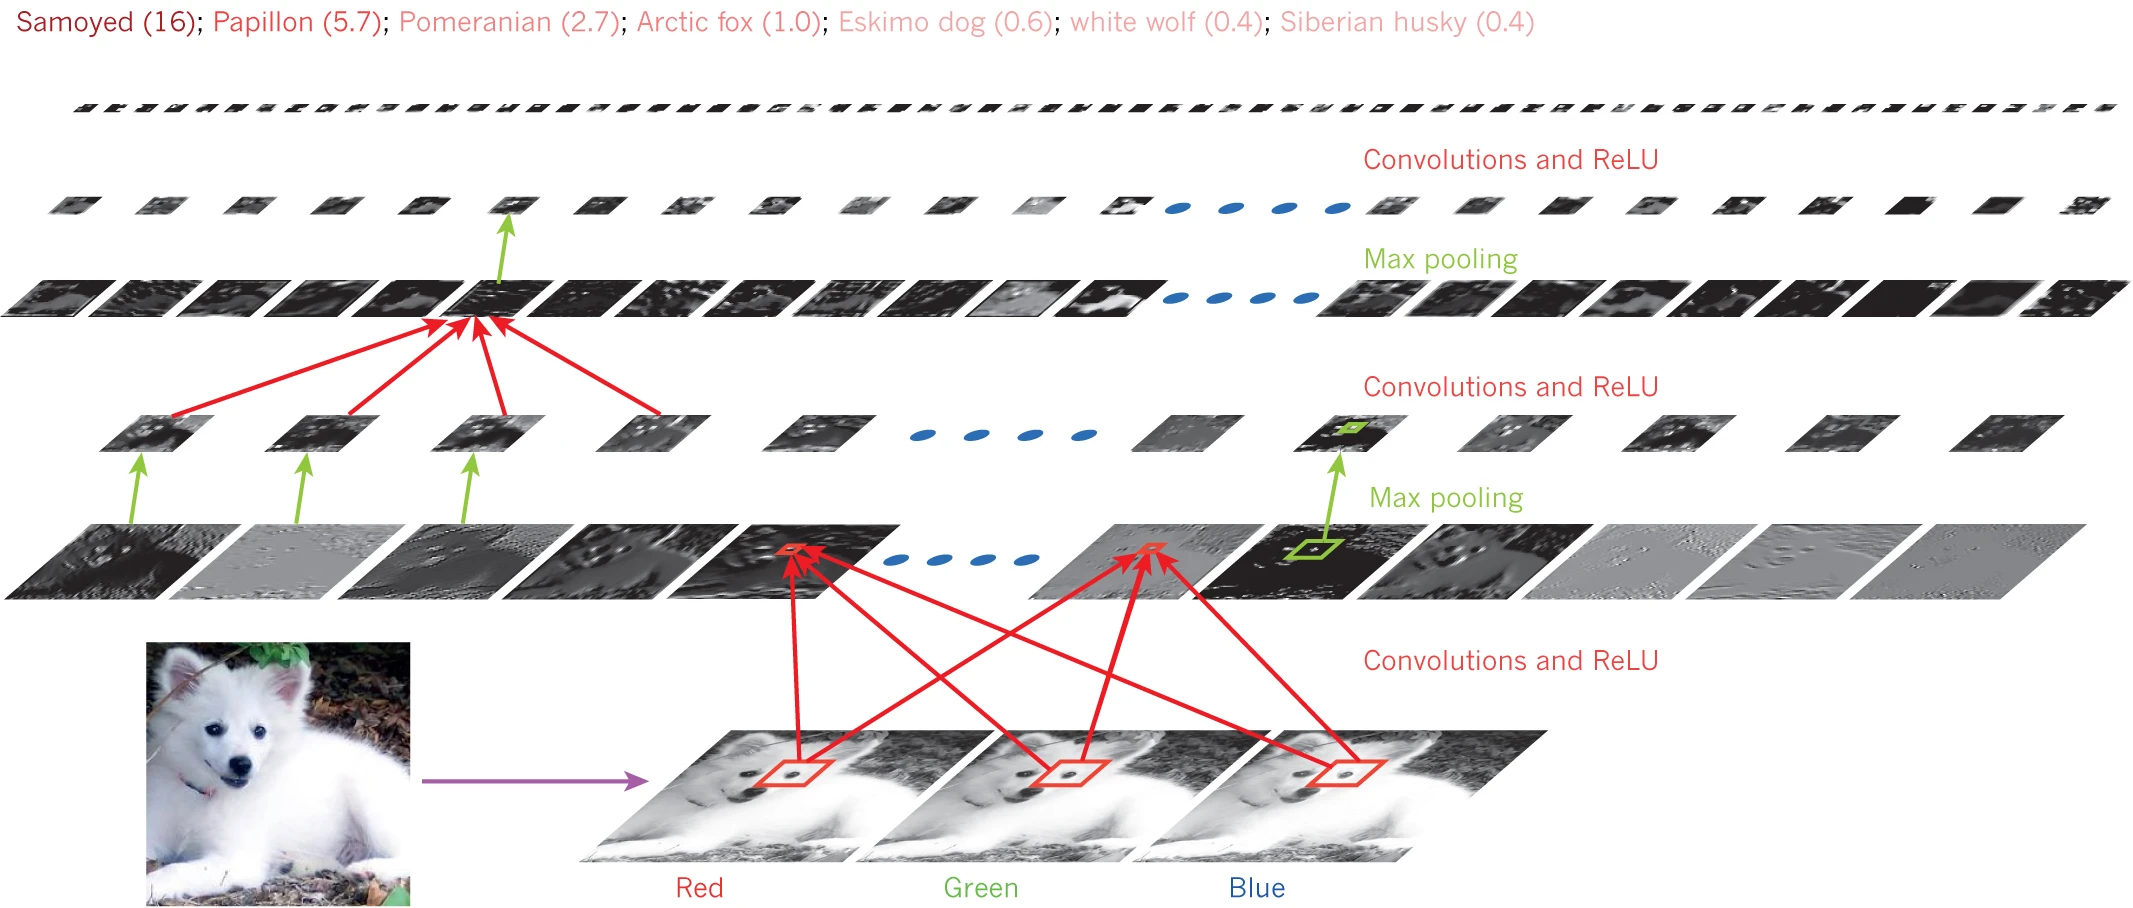
\includegraphics[width = \linewidth]{float/ch.intro/lecun.png}
        \caption*{卷积神经网络图像分类模型示例(引用于Lecun et al. “Deep Learning.” Nature, 2015, 521.7553: 436-444)}
    \end{figure}

\end{frame}

\begin{frame}
    \frametitle{模型选择问题}

    对于由超参数\(\vartheta\)和权重参数\(\theta\)所定义的深度学习预测模型\(f\),其模型选择问题便是如何选择合适的\(\vartheta\)与\(\theta\)从而提升模型\(f\)预测性能的问题。

    \begin{itemize}
        \item 权重参数\(\theta\)的优化研究 \(\rightarrow\) 梯度下降方法的改进
        \item 超参数\(\vartheta\)的优化研究 \(\rightarrow\) 神经网络结构的优化
    \end{itemize}

    \vspace{0.5em}
    神经网络结构的分解:
    \begin{itemize}
        \item 表征结构
        \begin{itemize}
            \item 隐藏结构 \(\rightarrow\) 神经网络结构搜索 (NAS)
                \begin{itemize}
                    \item 启发式优化、强化学习 \(\rightarrow\) 计算开销大,选择耗时长
                \end{itemize}
            \item 输入结构 \(\rightarrow\) 预测领域的多输入特征选择
            \begin{itemize}
                \item 封装法更优 \(\rightarrow\) 多时步维度的输入特征结构
            \end{itemize}
        \end{itemize}
        \item 输出结构 \(\rightarrow\) 预测领域的多输出策略优化
 \begin{itemize}
            \item MIMO策略,Direct策略,Iterative策略
            \begin{itemize}
                \item MIMO更优 \(\rightarrow\) MIMO策略下依然存在多种输出结构
            \end{itemize}
        \end{itemize}
    \end{itemize}

\end{frame}

\begin{frame}
    \frametitle{模型选择研究}

    \(\theta\)依赖于超参数\(\vartheta\):
    \begin{itemize}
        \item 模型神经网络结构参数(如CNN模型中卷积层层数、卷积核宽度和卷积核数量等等)
        \item 梯度下降方法参数(如SGD方法中的学习速率、批次样本选取数量和动量惯性系数等等)
    \end{itemize}

    \begin{center}
        不同的\(\vartheta\)必然会导致\(\theta\)的差异
    \end{center}

\end{frame}

\begin{frame}
    \frametitle{模型选择过程}
\begin{algorithm}[H]
    \caption{基于梯度下降方法的神经网络预测建模技术模型选择过程}
    \begin{algorithmic}[1]

        \WHILE{未满足模型选择方法界定的收敛条件}
        \STATE \(j\leftarrow j+1\)
        \STATE 从超参数集合\(\vartheta\)的搜索空间\(\Omega\)中选择或更新出当前的超参数集合\(\vartheta^j\)
        \STATE 基于\(\vartheta^j\):\\
        \hspace{2em}执行梯度下降算法所示步骤\\
        \hspace{2em}得到当前\(\vartheta^j\)试验下的权重参数集合\(\theta|\vartheta^j\)\\
        \hspace{2em}确定模型\(f \leftarrow  f \in \{\vartheta^j, \theta|\vartheta^j\}\)
        \STATE 基于数据集\(\mathd\)和模型\(f\),计算模型误差
        \STATE 基于模型误差与超参数更新方法:\\
        \hspace{2em}更新最优的神经网络超参数集合\(\vartheta^*\)\\
        \hspace{2em}更新最优的神经网络超参数集合\(\theta^* \leftarrow  \theta|\vartheta^*\)
        \ENDWHILE
        \RETURN {
            已完成更新过程的超参数集合\(\vartheta \leftarrow \vartheta^*\)与权重参数集合\(\theta \leftarrow \theta^*\)
        }
    \end{algorithmic}
\end{algorithm}   

\end{frame}

\begin{frame}{模型选择挑战}
    \begin{figure}
        \begin{minipage}[b]{0.45\textwidth}
            深度学习预测建模技术所面临的模型选择挑战尤为突出。
            \vspace{2em}
            \begin{itemize}
                \item 更多的权重参数以及更加复杂的梯度计算方式,导致模型选择效率低
                \item 复杂的神经网络结构加深了超参数搜索空间的复杂程度,导致模型选择效果弱
            \end{itemize}
        \end{minipage}
        \quad
    \begin{minipage}[b]{0.45\textwidth}
        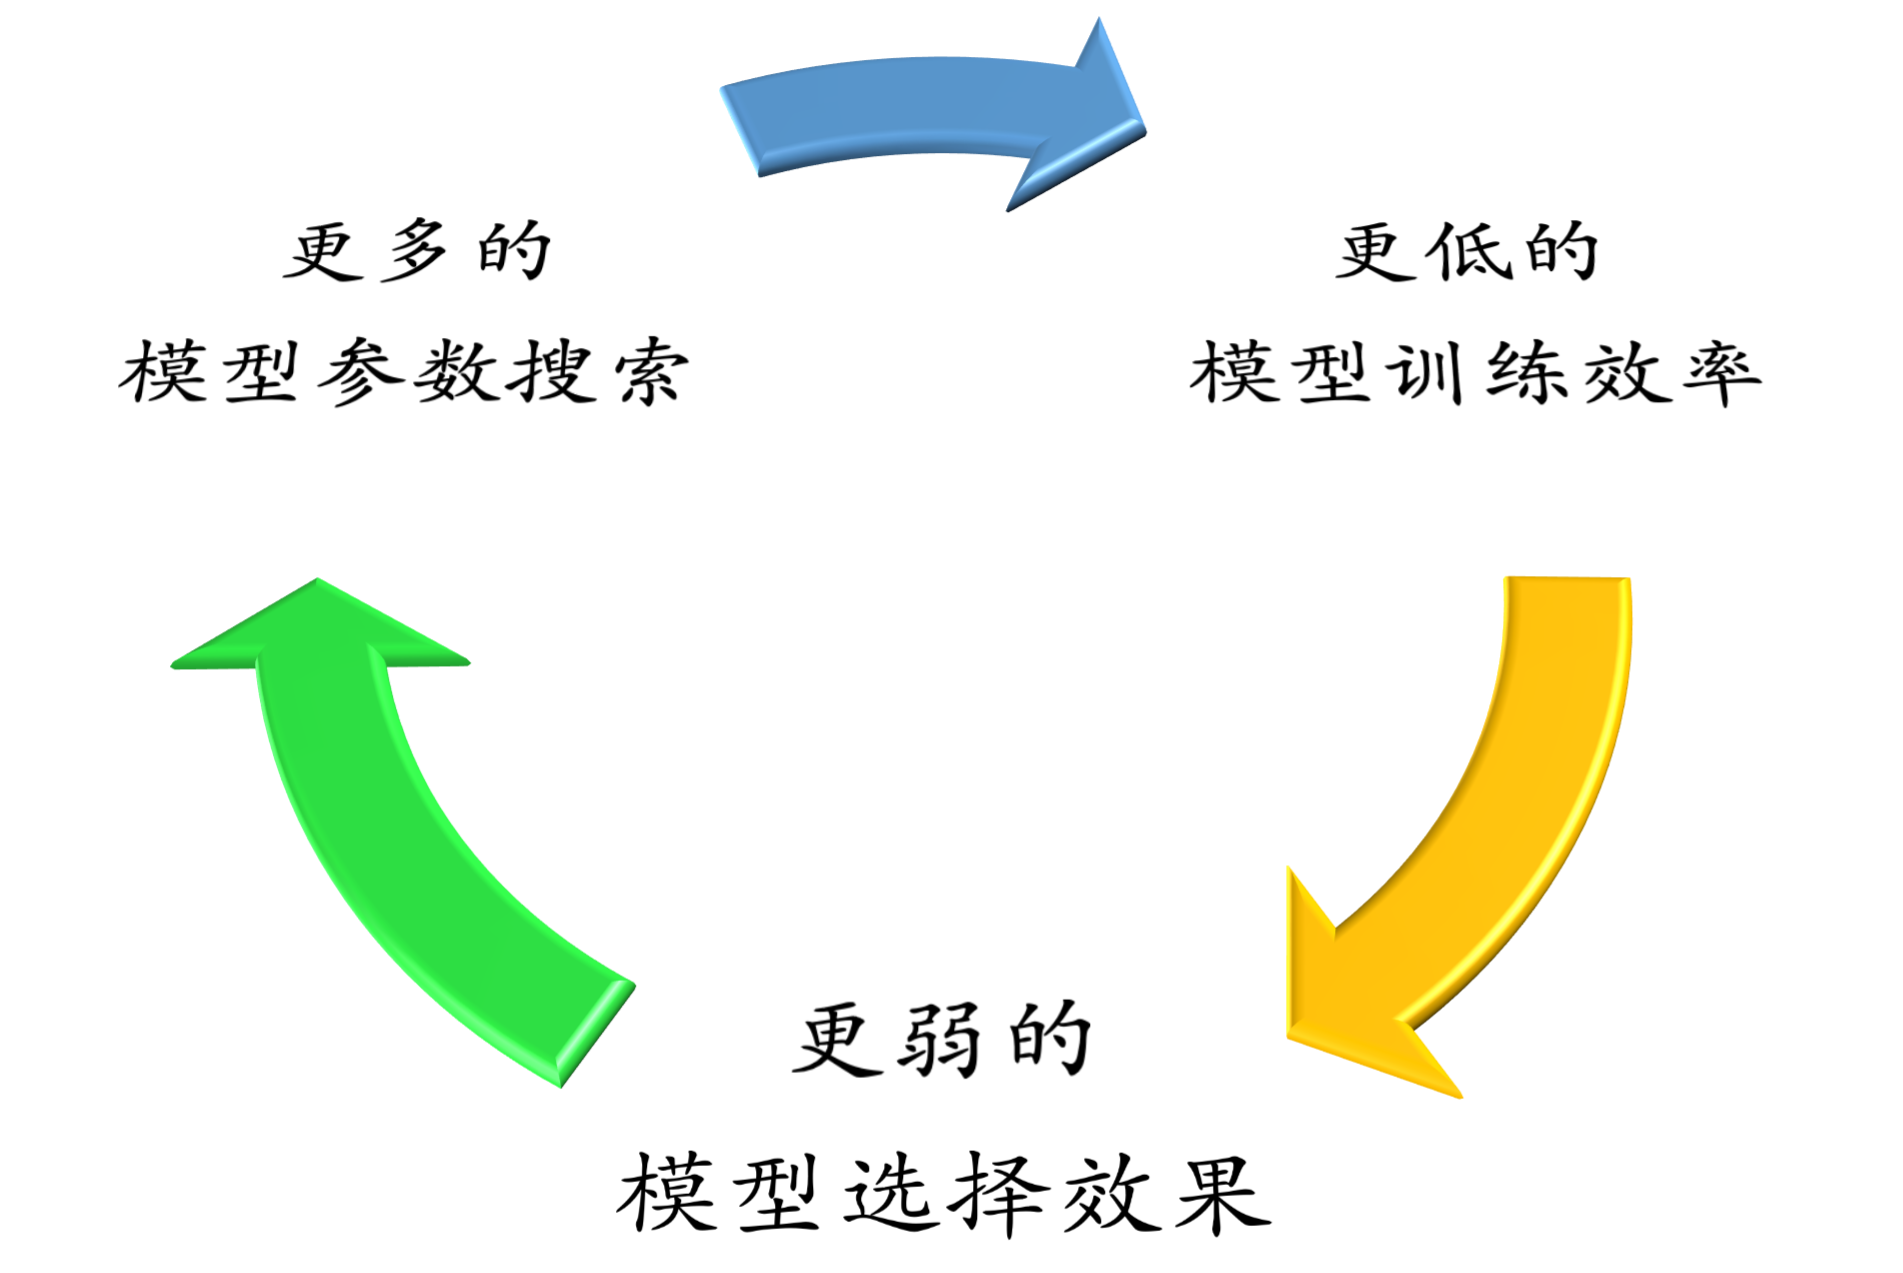
\includegraphics[width=\textwidth]{float/ch.intro/circle.png}
    \end{minipage}
    \end{figure}
    \end{frame}

    \begin{frame}
        \frametitle{随机映射方法研究概况}
        随机映射是一种采用非迭代学习机制的MLP建模方法。
    
        \begin{figure}[H]
            \begin{subfigure}[b]{0.25\textwidth}
                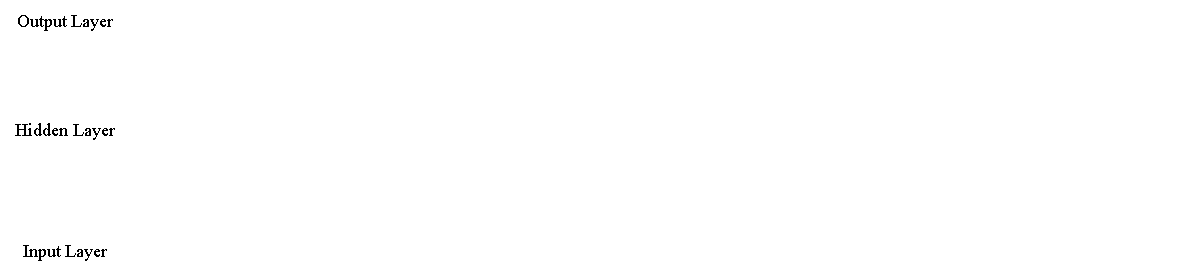
\includegraphics[height=\linewidth]{float/ch.cnn/layer.pdf}
                \caption*{}
            \end{subfigure}
            \hspace*{-0.15\textwidth}
            \begin{subfigure}[b]{0.25\textwidth}
                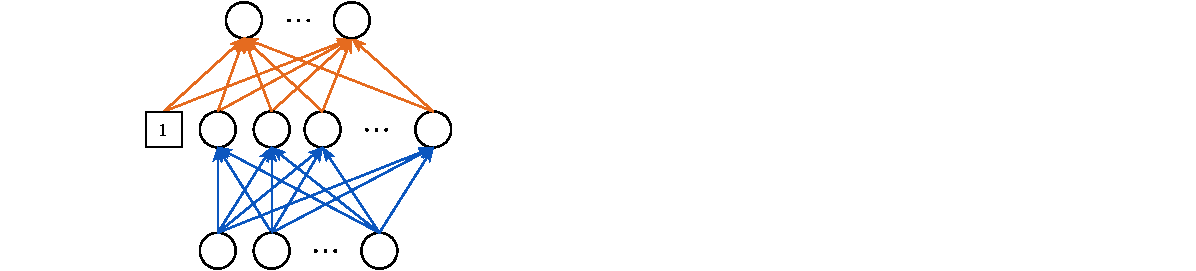
\includegraphics[height=\linewidth]{float/ch.cnn/schmidt.pdf}
                \caption{Schimidt网络}
            \end{subfigure}
            \hspace*{0.03\textwidth}
            \begin{subfigure}[b]{0.25\textwidth}
                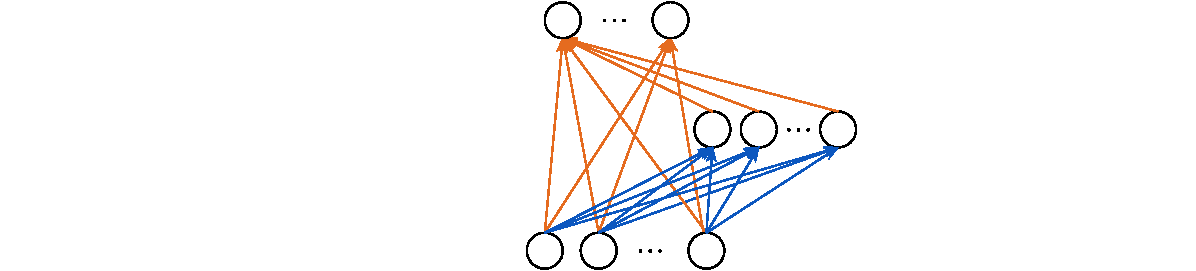
\includegraphics[height=\linewidth]{float/ch.cnn/rvfl.pdf}
                \caption{RVFL网络}
            \end{subfigure}
            \hspace*{\fill}
            \begin{subfigure}[b]{0.25\textwidth}
                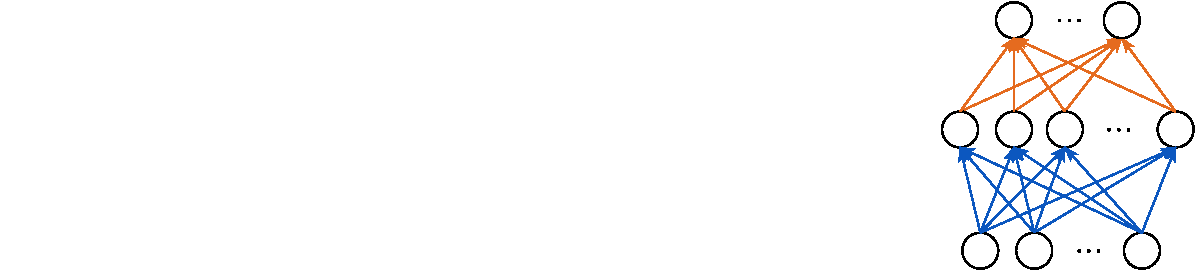
\includegraphics[height=\linewidth]{float/ch.cnn/elm.pdf}
                \caption{ELM网络}
            \end{subfigure}
            \caption*{\label{fig:randomnet}蓝色线表示固定的随机初始化权重,黄色线表示闭式求解得输出权重。}
        \end{figure}
        
    \end{frame}

    \begin{frame}
        \frametitle{随机映射建模过程}
    
        以MLP为例:随机映射多层感知机(Stochastic multiple percentage, SMLP)模型的预测过程为:
        \begin{align*}
            f_{smlp}(\x) &= \w_{out}\h_{smlp}, \\
            \h_{smlp} &= \sigma (\w_{hid}\x). \notag
        \end{align*}
        其模型损失函数依然保持MSE损失形式
        \begin{align*}
            \w_{out} &= \argmin_{\w_{out}} \norm{\y - \w_{out}\h_{smlp}} \\ 
            & = \y \h_{smlp}^{\trans} (\h_{smlp}\h_{smlp}^\trans)^{-1}. \notag
        \end{align*}
    
        支持向量机模型是一种SMLP模型的特例
    \end{frame}

    \begin{frame}
        \frametitle{SMLP的收敛性质}
    
        传统的SMLP模型避免了梯度下降训练计算开销高的问题,但这种权重随机机制使其模型性能的收敛性与稳定性受到质疑。
    
        针对于此:
        \begin{itemize}
            \item Huang等\footnote{Huang et al. "Universal approximation using incremental constructive feedforward networks with random hidden nodes." IEEE Trans. Neural Networks 17.4 (2006): 879-892.}基于递归添加神经元的方式构造了一种增长极限感知机(Incremental extreme learning machine,IELM),并证明了IELM对于任意连续有界目标函数的学习收敛能力。
            \item Wang等\footnote{Wang et al. "Stochastic configuration networks: Fundamentals and algorithms." IEEE transactions on cybernetics 47.10 (2017): 3466-3479.}通过迭代增加隐藏层神经元,基于监督机制闭式挑选神经元隐藏层权重,全局更新输出层权重的方式,构造出增长的SMLP模型,并证明了SCN的普适逼近性质(Universal approximation property)。
        \end{itemize}
        
    \end{frame}

    \begin{frame}
        \frametitle{随机映射深度学习建模技术}
    
        随机映射RNN的研究:
        \begin{itemize}
            \item Jaeger等\footnote{Jaeger et al. "Harnessing nonlinearity: Predicting chaotic systems and saving energy in wireless communication." science 304.5667 (2004): 78-80.}在2001年提出随机映射RNN,称其为状态回声网络(Echo state network,ESN)。
            \item 技术:Leaky ESN,Growing ESN,Deep ESN,Regularize ESN
            \item 应用:电力负荷预测,原油价格预测
        \end{itemize}
    
        随机映射CNN的研究:
        \begin{itemize}
            \item He等\footnote{He et al. "A powerful generative model using random weights for the deep image representation." Advances in Neural Information Processing Systems 29 (2016).}发现随机映射CNN在纹理生成和风格迁移等任务上具有不亚于梯度下降训练CNN的表现。
            \item 预测研究较少
        \end{itemize} 
    \end{frame}

    \begin{frame}
        \frametitle{随机映射深度学习预测建模技术}
    
        由此,针对时间序列深度学习预测技术模型选择挑战中的低效问题,构造基于随机映射的深度学习预测建模技术是一种有效的解决途径
        \begin{itemize}
            \item 深度学习建模技术优异的预测潜能
            \item 随机映射建模技术高效的建模效率
        \end{itemize}
    
        \vspace{1em}
        随机映射深度学习预测建模技术的挑战:
        \begin{itemize}
            \item 建模效率的提高建立在预测性能的牺牲上
            \item 更高的模型选择要求
        \end{itemize}
    
    \end{frame}


\begin{frame}
    \frametitle{技术研究体系}
\vspace{-0.5em}
\centering
\begin{figure}[!th]
    \centering
    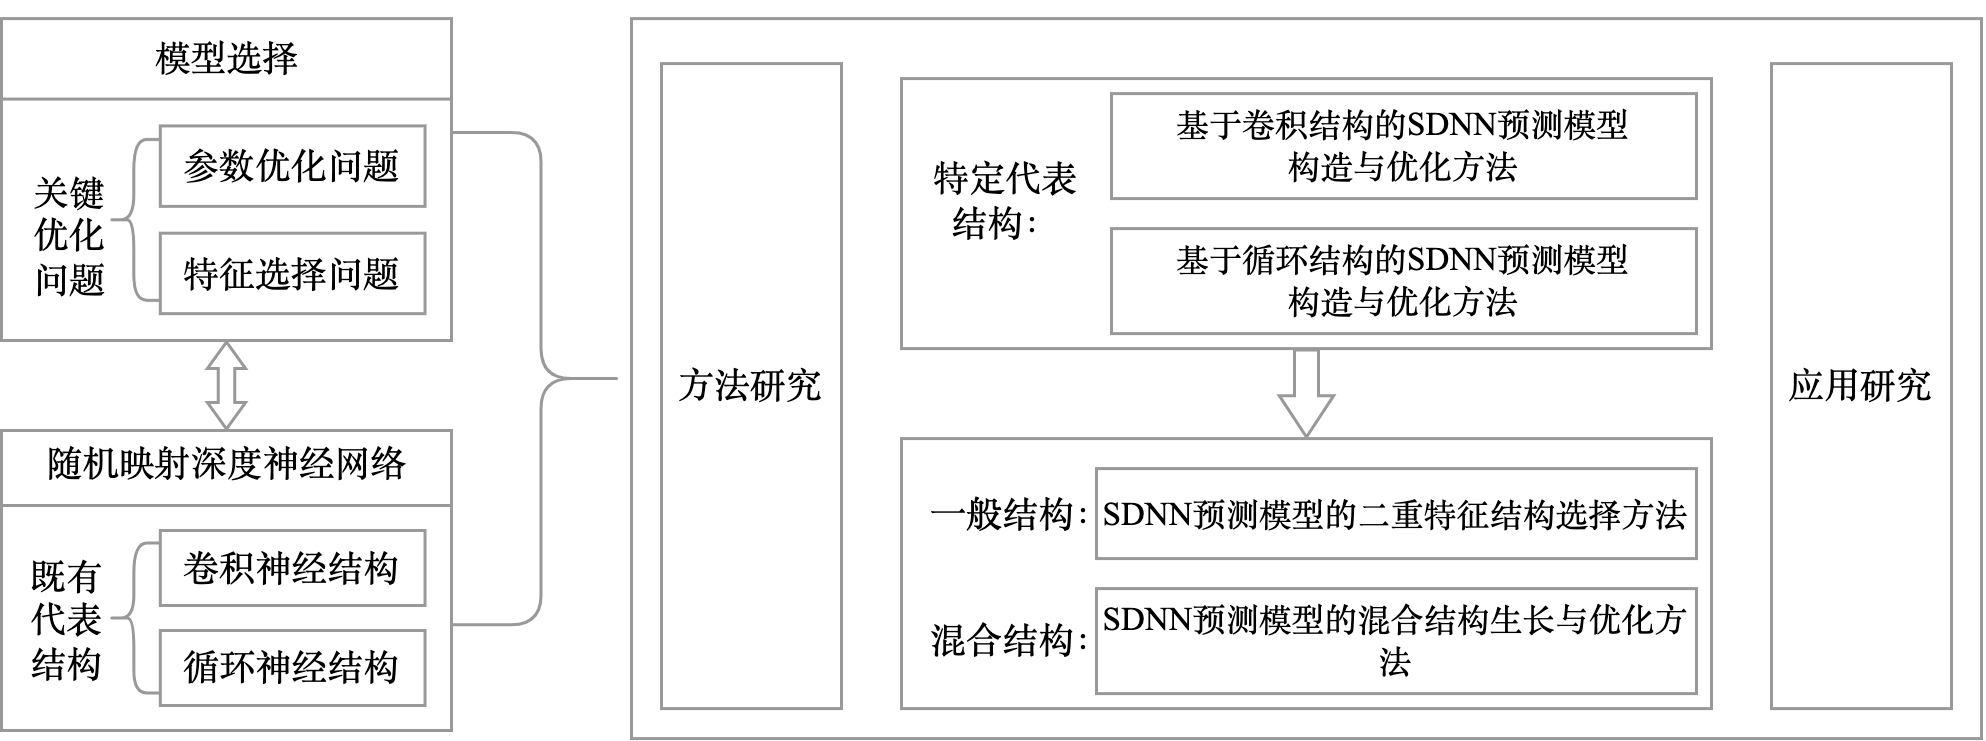
\includegraphics[width=0.88\linewidth]{float/ch.intro/thesis.png}
    
\end{figure}
\end{frame}

\begin{frame}
    \frametitle{研究意义}

    \textbullet ~~~ 在理论层面,本论文将深入研究不同神经网络结构下的SDNN预测模型和新的理论分析框架,如构建基于卷积结构和混合结构的SDNN预测模型的预测误差收敛性分析框架,直观理解SDNN预测模型的构造与决策逻辑

    \textbullet ~~~在方法层面,本论文将构造多套预测模型构造与优化方法,包括适用于卷积结构、循环结构、一般结构至混合结构SDNN模型的优化技术,形成从特定到一般再到混合的综合技术体系与框架,为SDNN预测建模技术的复杂模型选择问题提供新颖的方法与思路

    \textbullet ~~~在现实层面,本论文将立足于现实时间序列预测任务的多个场景,包括公共卫生领域中的流感阳性样本率预测任务、能源市场中的原油价格预测任务、金融市场中的股票指数预测任务、大气污染中的PM2.5预测任务、电力系统中的电力负荷与电力价格预测任务等
    
\end{frame}